\makeatletter
\def\input@path{{./Graphics/}} % Définition du chemin d'entrée pour les graphiques
\makeatother

\documentclass[12pt,a4paper]{article} % Classe de document

% Chargement des packages essentiels
\usepackage[utf8]{inputenc} % Encodage UTF-8
\usepackage[french]{babel} % Support de la langue française
\usepackage{graphicx, amsthm, mathtools, amsfonts, amssymb, physics, longtable, mathrsfs} % Packages pour les graphiques et mathématiques

\usepackage{float} % Gère le placement des objets flottants
\floatplacement{figure}{H} % Forces les figures à être placées exactement à l'endroit où elles apparaissent dans le texte

\usepackage[svgnames,x11names,rgb,table]{xcolor} % Définit les couleurs par noms
\usepackage{array, multicol, wrapfig, lmodern, multirow, booktabs, chemformula} % Diverses améliorations de mise en forme
\usepackage[detect-all=true, group-minimum-digits=4]{siunitx} % Pour les unités SI

\usepackage[bf, textfont={footnotesize,it}]{caption} % Personnalisation des légendes

% Configuration des marges de la page
\usepackage[margin=2cm, a4paper]{geometry}

\usepackage{fancyvrb} % Remplacement du mode verbatim qui permet une meilleure mise en forme
%\usepackage[Export]{adjustbox} % Utilisé pour contraindre les images à une taille maximale
%\adjustboxset{max size={0.9\linewidth}{0.9\paperheight}} % Taille maximale des images

% Configuration pour hyperref
\usepackage{hyperref} 
\hypersetup{
    colorlinks=true, % Colorise les liens
    breaklinks=true, % Permet le retour à la ligne dans les liens trop longs
    allcolors=Blue3, % Couleur des liens
    pdfauthor={Nana Engo}, % Auteur du document PDF
    pdfsubject={Chimie quantique et VQE}, % Sujet du document
    pdftitle={PHY4268 - Chimie quantique et VQE V25.03}, % Titre du document
    bookmarksopen=true % Ouvre les signets PDF par défaut
}

\usepackage{cleveref} % Améliore la gestion des références croisées

\frenchbsetup{StandardLayout=true} % Configuration du layout français
\numberwithin{equation}{section} % Numérotation des équations par section
\numberwithin{figure}{section} % Numérotation des figures par section
\numberwithin{table}{section} % Numérotation des tables par section

\setcounter{secnumdepth}{3} % Pour inclure les sous-sections
\renewcommand{\thesection}{\arabic{section}} % Numérotation des sections
%
\newcommand{\tcb}[1]{\textcolor{blue}{#1}} % textcolor{blue}{#1}
\newcommand{\tcr}[1]{\textcolor{red}{#1}} % textcolor{red}{#1}
% Titre du document
\title{\vspace*{8cm}
\large\tcb{Chapter 1 - Quantum Chemistry Modelling Basis}
\vspace*{5cm}}

\author{
\begin{tabular}{lr}
    \textbf{Nana Engo} & \textbf{Tchapet Njafa}\\
    {\small  serge.nana-engo@facsciences-uy1.cm} &\hspace*{2em}
    {\small jean-pierre.tchapet@facsciences-uy1.cm}
\end{tabular}\\[3em] % Espace entre les auteurs et la filiation
\textit{Quantum Simulation Group}\\
    \textit{Department of Physics} \\ 
    \textit{Faculty of Science} \\ 
    \textit{University of Yaoundé I}
}
\date{\vspace*{3cm}March 2025} % Date du document

\begin{document}
\maketitle % Affiche le titre, les auteurs et la date

% Espace supplémentaire après le titre (ajustable si nécessaire)
%\vspace*{2cm}

\newpage
\section{Introduction}

La chimie quantique est une discipline fondamentale qui permet de décrire et de prédire les propriétés électroniques et structurales des systèmes atomiques et moléculaires à l'aide des principes de la physique quantique. Elle constitue un outil essentiel pour comprendre les interactions chimiques, modéliser les réactions complexes et développer des applications pratiques dans des domaines variés tels que la conception de nouveaux matériaux, l'optimisation des processus chimiques ou encore le développement de médicaments.

Avec l'émergence des technologies computationnelles modernes et des algorithmes avancés comme le \emph{Variationnel Quantum Eigensolver} (VQE), la chimie quantique computationnelle a révolutionné la recherche scientifique et industrielle. Ces approches permettent de simuler efficacement des systèmes complexes en exploitant des approximations telles que l'approximation de Born-Oppenheimer (BO) ou la méthode Hartree-Fock (HF), tout en maintenant un équilibre entre précision et faisabilité computationnelle.

Dans ce chapitre, nous introduisons les concepts fondamentaux suivants :
\begin{itemize}
    \item L'Hamiltonien moléculaire en première quantification ;
    \item L'approximation de Born-Oppenheimer ;
    \item L'approche du champ moyen via la méthode Hartree-Fock (HF) ;
    \item Les limites inhérentes à cette méthode ;
    \item Le choix et l'importance des ensembles de bases.
\end{itemize}

Ces notions sont illustrées par leur rôle dans le workflow de l'algorithme VQE (voir les encadrées en rouge sur la \autoref{fig:VQE_Flowchart}), qui constitue une avancée majeure pour les simulations moléculaires en chimie quantique. Ces méthodes ont de nombreuses applications pratiques, notamment dans le domaine énergétique (\autoref{fig:CoverVQE}) , où elles contribuent au développement de matériaux innovants et à l'optimisation des processus chimiques.

Ce chapitre vise à fournir une base solide pour comprendre les principes sous-jacents à la modélisation chimique en physique quantique, tout en mettant en lumière les défis computationnels et les opportunités offertes par ces approches modernes.

\begin{figure}
\centering

\includegraphics[width=.9\linewidth]{VQE_Flowchart.jpeg} 
\caption{\textbf{Diagramme de flux de l'algorithme VQE (Variationnel Quantum Eigensolver).} Ce diagramme illustre les étapes principales de l'algorithme VQE, une méthode hybride quantique-classique utilisée pour calculer l'énergie des molécules. On y voit comment une boucle itérative optimise les paramètres d'un circuit quantique (ansatz) afin de minimiser l'énergie, en utilisant un calculateur classique pour le contrôle et l'analyse des résultats quantiques. Les encadrés rouges mettent en évidence les contributions des concepts fondamentaux présentés dans ce chapitre, comme l'Hamiltonien moléculaire et l'approximation de Born-Oppenheimer.}
\label{fig:VQE_Flowchart}
\end{figure}

\begin{figure}
\centering

\includegraphics[width=.4\linewidth]{CoverVQE.jpg}
\caption{\textbf{Applications de la chimie quantique computationnelle dans le domaine de l'énergie.} Parmi celles-ci, on retrouve la conception de nouveaux matériaux pour les cellules solaires, l'optimisation des réactions catalytiques pour la production d'énergie propre, le développement de batteries plus performantes et la compréhension des mécanismes de stockage de l'énergie. Ces applications montrent le potentiel de la chimie quantique pour résoudre les défis énergétiques actuels.}
\label{fig:CoverVQE}
\end{figure}

\section{Hamiltonien moléculaire en première quantification}

\begin{figure}
\centering

\includegraphics[width=0.7\linewidth]{Interaction_QC.pdf}
\caption{\textbf{Illustration simplifiée des différentes interactions dans un système moléculaire.} Ce diagramme schématise les interactions fondamentales présentes dans une molécule, incluant les attractions et répulsions électrostatiques. On distingue les interactions entre les électrons et les noyaux (attraction), les répulsions entre les électrons, et les répulsions entre les noyaux. Les étiquettes sur le schéma mettent en évidence la nature Coulombienne de ces interactions et montrent comment ces forces contribuent à l'énergie totale du système. La figure aide à visualiser les composantes de l'Hamiltonien moléculaire avant l'application de l'approximation de Born-Oppenheimer.}
\label{fig:interactionqc}
\end{figure}

En chimie quantique, l'équation de Schrödinger joue un rôle central dans la description des systèmes atomiques et moléculaires. La forme générale de l'équation de Schrödinger dépendante du temps est :\begin{equation}
i\hbar \pdv{t} |\psi(t)\rangle = \mathtt{H} |\psi(t)\rangle .
\end{equation}
$|\psi(t)\rangle$ représente la fonction d'état du système, décrivant son évolution temporelle, et $\mathtt{H}$ est l'opérateur Hamiltonien, qui représente l'énergie totale du système. Résoudre cette équation directement, même en l'absence d'effets relativistes, reste un défi majeur pour les systèmes moléculaires complexes.

Pour simplifier, on se concentre souvent sur les états stationnaires du système. Ces états sont décrits par l'équation de Schrödinger indépendante du temps, qui prend la forme d'un problème aux valeurs propres :
\begin{equation}
\mathtt{H} |\psi\rangle = E |\psi\rangle ,
\end{equation}
où $E$ représente l'énergie de l'état stationnaire $|\psi\rangle$. La résolution de cette équation nous permet de déterminer les énergies permises et les fonctions d'état associées à ces états.

L'Hamiltonien moléculaire, noté $\mathtt{H}$, décrit l'énergie totale d'une molécule constituée de $M$ noyaux et de $N$ électrons. Il englobe les énergies cinétiques et potentielles de toutes les particules en interaction. De manière générale, il peut être exprimé comme la somme des termes suivants (voir la \autoref{fig:interactionqc}):
\begin{equation}
\mathtt{H}=\mathtt{T}_e+\mathtt{T}_n+\mathtt{U}_{en}+\mathtt{U}_{en}+\mathtt{U}_{nn},
\end{equation}
où
\begin{itemize}
\item $\mathtt{T}_e= -\sum_i\frac{\hbar^2}{2m_e}\nabla^2_i$ est l'énergie cinétique électronique; 
\item $\mathtt{T}_n=-\sum_I\frac{\hbar^2}{2M_I}\nabla^2_I$ est l'énergie cinétique nucléaire; 
\item $\mathtt{U}_{en}= -\sum_{i,I}\frac{e^2}{4\pi\epsilon_0}\frac{Z_I}{|\mathbf{r}_i-\mathbf{R}_I|}$ est la répulsion Coulombienne entre les électrons et les noyaux; 
\item $\mathtt{U}_{ee}=+\frac{1}{2}\sum_{i\neq j}\frac{e^2}{4\pi\epsilon_0}\frac{1}{|\mathbf{r}_i-\mathbf{r}_j|}$ est la répulsion Coulombienne entre les électrons eux-mêmes; 
\item $\mathtt{U}_{nn}=+\frac{1}{2}\sum_{I\neq J}\frac{e^2}{4\pi\epsilon_0}\frac{Z_IZ_J}{|\mathbf{R}_I-\mathbf{R}_J|}$ est la répulsion Coulombienne entre les noyaux eux-mêmes.
\end{itemize}
Dans ces expressions, $i$ et $j$ sont des indices qui parcourent tous les électrons, tandis que $I$ et $J$ parcourent tous les noyaux. Les variables $M_I$, $\mathbf{R}_I$, et $Z_I$ désignent respectivement la masse, la position et le numéro atomique du \emph{I}-ième noyau, tandis que $\mathbf{r}_i$ est la position du \emph{i}-ième électron.

Pour simplifier les calculs et faciliter l'interprétation des résultats, il est courant de travailler en unités atomiques. Dans ce système d'unités, l'unité de longueur est le Bohr ($a_0 \approx \SI{0.529167e-10}{\meter}$), l'unité de masse est la masse de l'électron ($m_e$), et l'unité d'énergie est le Hartree (\SI{1}{Hartree} $= \frac{e^2}{4\pi\epsilon_0 a_0} \approx \SI{27.2113}{\electronvolt}$). L'utilisation de ces unités simplifie les équations en fixant certaines constantes physiques à 1.

En définissant $M_I' = M_I / m_e$, les différents termes de l'Hamiltonien moléculaire s'expriment en unités atomiques comme suit :
\begin{equation}
\begin{split}
\mathtt{T}_e&=-\sum_i\frac{\nabla^2_i}{2}, \qquad\mathtt{T}_n= -\sum_I\frac{\nabla^2_I}{2M_I'}, 
 \qquad\mathtt{U}_{en}= - \sum_{i,I}\frac{Z_I}{|\mathbf{r}_i-\mathbf{R}_I|},\\
\mathtt{U}_{ee}&=+\frac12\sum_{i\neq j}\frac{1}{|\mathbf{r}_i-\mathbf{r}_j|}
=+\sum_{i,j>i}\frac{1}{|\mathbf{r}_i-\mathbf{r}_j|}=+\sum_{i,j>i}\frac{1}{r_{ij}},\\
\mathtt{U}_{nn}&=+\frac12\sum_{I\neq J}\frac{Z_IZ_J}{|\mathbf{R}_I-\mathbf{R}_J|}
=+\sum_{I,J>I}\frac{Z_IZ_J}{|\mathbf{R}_I-\mathbf{R}_J|}=+\sum_{I,J>I}\frac{Z_IZ_J}{R_{IJ}}.
\end{split}
\end{equation}

Cependant, la résolution directe de l'équation de Schrödinger avec cette Hamiltonien complet est extrêmement complexe, voire impossible, pour les systèmes moléculaires de taille significative. Cette complexité découle des interactions corrélées entre les nombreux électrons et noyaux. Pour surmonter cette difficulté, des approximations sont indispensables.

\section{Approximation de Born-Oppenheimer}\label{approximation-de-born-oppenheimer}

L'\textbf{approximation de Born-Oppenheimer} est une hypothèse fondamentale en chimie quantique, qui simplifie considérablement le traitement des systèmes moléculaires complexes. Elle repose sur la différence significative de masse entre les noyaux et les électrons. Les noyaux, étant bien plus massifs que les électrons ($M'\sim10^3$), se déplacent beaucoup plus lentement. Cette disparité dynamique permet de séparer les mouvements électroniques et nucléaires lors de la résolution de l'équation de Schrödinger (voir la \autoref{fig:bointeractionqc}). En d'autres termes, on considère que les électrons s'adaptent instantanément aux mouvements des noyaux, ce qui permet de découpler leurs équations de mouvement.

\begin{figure}
\centering

\includegraphics[width=0.7\linewidth]{BO_Interaction_QC.pdf}
\caption{\textbf{Illustration des interactions dams l'approximation de Born-Oppenheimer.} Ce schéma met en évidence la séparation des mouvements rapides des électrons et des mouvements lents des noyaux, due à la grande différence de masse entre ces particules. Les électrons sont considérés comme se déplaçant dans un champ créé par les noyaux fixes, ce qui permet de simplifier considérablement les calculs de structure électronique.
}
\label{fig:bointeractionqc}
\end{figure}

\subsection{Hamiltonien réduit}

En appliquant cette approximation, le terme d'énergie cinétique nucléaire $T_n$ est négligé. De plus, l'énergie de répulsion nucléaire $\mathtt{U}_{nn}(\mathbf{R})$ devient constante pour une géométrie nucléaire donnée.  L'Hamiltonien électronique est alors extrait de l'Hamiltonien total:
\begin{equation}
\begin{split}
\mathtt{H}_{\text{elec}}(\mathbf{R}) &= \underset{\text{One-Electron Operators}}{\mathtt{T}_e + \mathtt{U}_{en}(\mathbf{R})} + \underset{\text{Two-Electron Operator}}{\mathtt{U}_{ee}}\\
&= \underset{\text{One-Electron Operator}}{\sum_i h(i)} + \underset{\text{Two-Electron Operator}}{\sum_{i\ne j}v(i, j)}\\
&=-\sum_{i=1}^N \frac12 \nabla_i^2 - \sum_{i=1}^N \sum_{A=1}^M \frac{Z_A}{r_{iA}} + \sum_{i=1}^N \sum_{j>i} \frac{1}{r_{ij}} .
\end{split}
\end{equation}
Cet Hamiltonien électronique dépend explicitement des positions des électrons, mais les positions des noyaux y apparaissent uniquement comme des paramètres fixes. Pour une configuration nucléaire donnée, on peut donc calculer l'énergie électronique $(E_{\text{elec}})$ en résolvant l'équation de Schrödinger électronique :
\begin{equation}
\mathtt{H}_{\text{elec}}(\mathbf{R}) \psi_{\text{elec}}(\mathbf{r}; \mathbf{R}) = E_{\text{elec}}(\mathbf{R}) \psi_{\text{elec}}(\mathbf{r}; \mathbf{R})
\end{equation}
où $\psi_{\text{elec}}(\mathbf{r}; \mathbf{R})$ est la fonction d'état électronique qui dépend des coordonnées électroniques ($\mathbf{r}$) et paramétriquement des coordonnées nucléaires ($\mathbf{R}$).

\subsection{Énergie totale du système}

La résolution de l'équation de Schrödinger électronique pour différentes configurations nucléaires permet de construire la \textbf{surface d'énergie potentielle (PES, Potential energy surface)}, $E_{\text{elec}}(\mathbf{R})$. Cette surface décrit l'énergie du système en fonction des positions des noyaux et est un concept central en chimie quantique.

Une fois l'énergie électronique obtenue, l'énergie totale est approchée comme suit :
\begin{equation}
E_{\text{tot}} = E_{\text{elec}} + E_{nn},
\end{equation}
où,
\begin{itemize}
\item $E_{\text{elec}}$ est l'énergie électronique, obtenue par la résolution de l'équation de Schrödinger électronique;
\item $E_{nn}=\sum_{A=1}^M \sum_{B>A} \frac{Z_A Z_B}{R_{AB}}$ représente l'énergie de répulsion entre les noyaux, considérés comme des charges ponctuelles fixes.
\end{itemize}

\subsection{Conséquences de l'approximation}

L'approximation de Born-Oppenheimer a des implications importantes :

\begin{itemize}
\item L'énergie totale est calculée pour une géométrie nucléaire fixe.  Cette simplification permet de déterminer les structures moléculaires à l'équilibre en minimisant l'énergie totale par rapport aux positions des noyaux.
\item Les mouvements des noyaux (vibration, rotation, translation) peuvent être traités séparément en utilisant un Hamiltonien nucléaire effectif :
\begin{equation}
\mathtt{H}_{\text{nucl}} = \mathtt{T}_n + E_{\text{tot}}(\{R_A\}) ,
\end{equation}
où $E_{\text{tot}}(\{R_A\})$ agit comme un potentiel pour le mouvement des noyaux. Ceci permet d'étudier les spectres vibrationnels des molécules.
\end{itemize}

En résumé, l'approximation de Born-Oppenheimer est essentielle pour séparer les degrés de liberté nucléaires et électroniques, rendant ainsi le problème beaucoup plus gérable en chimie quantique computationnelle.  Bien qu'elle repose sur une simplification, elle fournit une base solide pour la compréhension et la prédiction des propriétés moléculaires. Il est important de noter que cette approximation peut devenir moins précise dans certaines situations, notamment lorsque les surfaces d'énergie potentielle sont proches ou lorsqu'on étudie des processus dynamiques où le couplage entre les mouvements électroniques et nucléaires devient important.

\section{Méthode de Hartree-Fock - Approche du champ moyen}

La méthode de Hartree-Fock (HF) est une approche fondamentale qui approxime l'interaction électron-électron dans un système moléculaire en chimie quantique computationnelle. Elle introduit le concept de champ moyen (\textbf{mean-field} en anglais), où \textbf{chaque électron interagit avec un potentiel moyen créé par l'ensemble des autres électrons}. Cette approche inclut les effets d'échange dus au principe de Pauli, mais néglige la \textbf{corrélation électronique dynamique}, ce qui constitue l'une de ses principales limites.

\subsection{Fonction d'état - Déterminant de Slater}

L'approximation centrale de la méthode HF consiste à représenter la fonction d'état multi-électronique par un \textbf{déterminant de Slater}, qui encode mathématiquement l'antisymétrie requise pour les fermions sont les électrons, particules de spin-$\frac12$. Il est défini comme suit :
\begin{equation}
\begin{split}
\psi(\mathbf{r}_0, \mathbf{r}_1, \ldots, \mathbf{r}_{N-1})\equiv |\phi_{M-1},\cdots,  \phi_1, \phi_0 \rangle 
&=   \frac{1}{\sqrt{N!}}
\begin{vmatrix} \phi_0(\mathbf{r}_0) & \phi_1(\mathbf{r}_0) & \cdots & \phi_{M-1}(\mathbf{r}_0) \\
      \phi_0(\mathbf{r}_1) & \phi_1(\mathbf{r}_1) & \cdots & \phi_{M-1}(\mathbf{r}_1) \\
      \vdots & \vdots & \ddots & \vdots \\
      \phi_0(\mathbf{r}_{N-1}) & \phi_1(\mathbf{r}_{N-1}) & \cdots & \phi_{M-1}(\mathbf{r}_{N-1})
\end{vmatrix} \\
&\equiv |M-1,\dots, 1, 0 \rangle,
\end{split}
\end{equation} 
L'échange des positions de deux électrons est équivalent à l'échange de deux rangées du déterminant de Slater, ce qui modifie le signe de la fonction d'état. Cela fournit la symétrie d'échange correcte pour la fonction d'état fermionique. Bien que le nombre de spin-orbitales considérées, $M$, soit généralement plus élevé que le nombre d'électrons dans le système, $N$, les électrons ne peuvent occuper que $N$ des spin-orbitales dans un déterminant Slater donné. En conséquence, le déterminant de Slater ne contient que les spin-orbitales occupées $N$.

Dans la base des \textbf{orbitales moléculaires (MO)}, chaque fonction $\phi_i(\mathbf{r})$ est une combinaison linéaire des \textbf{orbitales atomiques (AO)} via la méthode \textbf{LCAO} :
\begin{equation}
\phi_i(\mathbf{r}) = \sum_{\mu} C_{\mu i} \chi_\mu(\mathbf{r} - \mathbf{R}_A),
\end{equation}
où $\chi_{\mu}(\mathbf{r})$ sont les fonctions de base et $C_{\mu i}$ les coefficients d’expansion.

\subsection{Exemple d'illustration}\label{exemple-dillustration}

Pour rendre les correspondances plus claires, nous examinons comment une fonction d'état sera représentée pour un système quantique fictif. On considère les orbitales de spin
$|A_\uparrow\rangle,\,|A_\downarrow\rangle,\,|B_\uparrow\rangle,\,|B_\downarrow\rangle$. Nous sommes libres de définir arbitrairement l'état Hartree-Fock de notre système fictif et de choisir les deux électrons dans l'orbitale $|A\rangle$. Nous sommes intéressés par la fonction d'état lorsque la composante $z$ du spin est nulle.

Labellisons chaque orbitale ainsi qu'il suit~:
\begin{align}
 &|A_\uparrow\rangle=|00\rangle=|\mathbf{0}\rangle,  &&|A_\downarrow\rangle=|01\rangle=|\mathbf{1}\rangle,
&&|B_\uparrow\rangle=|10\rangle=|\mathbf{2}\rangle,  &|B_\downarrow\rangle=|11\rangle=|\mathbf{3}\rangle.
\end{align}

L'état de Hartree-Fock possède les deux électrons dans les orbitales $|A\rangle$.
\begin{itemize}
\item Un état HF incorrectement symétrisé serait donc
\begin{equation}
|A_\uparrow\rangle_1|A_\downarrow\rangle_2 = |\mathbf{0}\rangle_1|\mathbf{1}\rangle_2,
\end{equation}
où les indices indiquent l'électron décrit par chaque orbitale.

\item La fonction d'état HF correctement antisymétrisée serait
\begin{equation}
\begin{split}
    |\Psi_{\mathrm{HF}}\rangle =  \frac{1}{\sqrt{2}}
        \begin{vmatrix}
        A_\uparrow(\mathbf{x}_0) & A_\downarrow(\mathbf{x}_0)\\
        A_\uparrow(\mathbf{x}_1) & A_\downarrow(\mathbf{x}_1)\\
        \end{vmatrix}
        &= \frac{1}{\sqrt{2}}  \Big( A_\uparrow(\mathbf{x_0}) A_\downarrow(\mathbf{x_1}) - A_\downarrow(\mathbf{x_0}) A_\uparrow(\mathbf{x_1})  \Big)\\
&=\frac{1}{\sqrt{2}} (|\mathbf{0}\rangle_1|\mathbf{1}\rangle_2 - |\mathbf{1}\rangle_1|\mathbf{0}\rangle_2 ).
\end{split}
\end{equation}
\end{itemize}

Si nous considérons maintenant les excitations au-dessus de l'état HF, alors une fonction d'état générale avec $s_z=0$ qui a été correctement antisymétrisée est donnée par
\begin{equation}
\begin{aligned}
|\Psi\rangle =& \frac{\alpha}{\sqrt{2}}(|\mathbf{0}\rangle_1|\mathbf{1}\rangle_2 - |\mathbf{1}\rangle_1|\mathbf{0}\rangle_2 ) 
+\frac{\beta}{\sqrt{2}} (|\mathbf{2}\rangle_1|\mathbf{3}\rangle_2 - |\mathbf{3}\rangle_1|\mathbf{2}\rangle_2 ) \\
+& \frac{\gamma}{\sqrt{2}} (|\mathbf{0}\rangle_1|\mathbf{3}\rangle_2 - |\mathbf{3}\rangle_1|\mathbf{0}\rangle_2 ) + \frac{\delta}{\sqrt{2}} (|\mathbf{1}\rangle_1|\mathbf{2}\rangle_2 - |\mathbf{2}\rangle_1|\mathbf{1}\rangle_2 ).
\end{aligned}
\end{equation}

\subsection{Approche variationnelle et opérateur de Fock}

L'énergie totale est obtenue par minimisation variationnelle, où l'énergie est exprimée comme fonction des orbitales. L'\textbf{opérateur de Fock} est introduit pour représenter le champ moyen ressenti par un électron :
\begin{equation}
F(d) = h + \sum_b \big(J_b(d) - K_b(d)\big) ,
\end{equation}
avec,
\begin{itemize}
\item $d$ une densité à N-électrons;
\item $h$ l'Hamiltonien à un électron (énergie cinétique et interaction électron-noyau);
\item  $J_b(d)$ le \textbf{terme de Coulomb}, représentant la répulsion classique,
    \begin{equation}
\begin{split}
        J_{ab} &:=\bra{\phi_a(\vb{r}_1)\phi_b(\vb{r}_2)}\frac{e^2}{\vb{r}_{12}}
        \ket{\phi_a(\vb{r}_1)\phi_b(\vb{r}_2)}\\
        &= \int \phi_a^*(\mathbf{r}_1) \phi_b^*(\mathbf{r}_2) \frac{e^2}{r_{12}} \phi_a(\mathbf{r}_1) \phi_b(\mathbf{r}_2) d\mathbf{r}_1 d\mathbf{r}_2,
\end{split}
    \end{equation}
\item $K_b(d)$ le \textbf{terme d’échange} à deux électrons, correction purement quantique,
    \begin{equation}
    \begin{split}
    K_{ab} & :=\bra{\phi_a(\vb{r}_1)\phi_b(\vb{r}_2)}\frac{e^2}{\vb{r}_{12}}
    \ket{\phi_a(\vb{r}_2)\phi_b(\vb{r}_1)}\\
    &= \int \phi_a^*(\mathbf{r}_1) \phi_b^*(\mathbf{r}_2) \frac{e^2}{r_{12}} \phi_b(\mathbf{r}_1) \phi_a(\mathbf{r}_2) d\mathbf{r}_1 d\mathbf{r}_2.
    \end{split}
    \end{equation}
\end{itemize}

Les orbitales sont optimisés de manière variationnelle pour un seul déterminant de Slater. En minimisant l'énergie totale, on obtient l'\textbf{équation de Hartree-Fock pour les orbitales moléculaires} :
\begin{equation}
F|\psi_a\rangle = \varepsilon_a|\psi_a\rangle .
\end{equation}
En exprimant les orbitales comme une combinaison linéaire finie de fonctions de base, cad en travaillant sur la base de la fonction de base centrée sur l'atome, cette équation devient l'\href{https://en.wikipedia.org/wiki/Roothaan_equations}{équation de Roothaan-Hall} :
\begin{equation}
\vb{F}\vb{C} = \vb{S}\vb{C}\varepsilon , 
\end{equation}
où,
\begin{itemize}
\item $\vb{F}$ est la matrice de Fock;
\item $\vb{C}$ est la matrice des coefficients orbitaux moléculaires;
\item $\vb{S}$ est la matrice de chevauchement/recouvrement des orbitales atomiques;
\item $\varepsilon$ est le vecteur des énergies des orbitales moléculaires.
\end{itemize}

\subsection{Procédure auto-cohérente (SCF)}

La méthode Hartree-Fock est résolue itérativement par une procédure auto-cohérente (Self-Consistent Field, SCF).

\begin{enumerate}
\item \textbf{Démarrage.} Initialisation des orbitales moléculaires avec une estimation $\vb{C}^{(0)}$. On founit les coordonnées 3D des atomes du système moléculaire.
\item \textbf{Construction de $\vb{F}$.} Calcul des matrices de Coulomb ($\vb{J}$) et d'échange ($\vb{K}$).
\item \textbf{Équation de Roothaan-Hall.} Diagonalisation de $\vb{F}$ pour obtenir les nouvelles orbitales et énergies.
\item \textbf{Mise à jour des orbitales.} Nouvelles orbitales $\vb{C}^{(k+1)}$ obtenues à partir de $\vb{F}$.
\item \textbf{Critère de convergence.} Comparer l'énergie $E^{(k+1)}$ avec $E^{(k)}$. Si $\big|E^{(k+1)} - E^{(k)}\big| < \delta$ (le seui), le processus est terminé.
\item \textbf{Retour en cas de non-convergence.} Si la convergence n'est pas atteinte, le cycle est répété.
\end{enumerate}

La \autoref{fig:scfworkflow} présente cette procédure sous forme de workflow.

\begin{figure}
\centering

\includegraphics[width=0.6\linewidth]{SCF_Workflow.pdf}
\caption{\textbf{Workflow détaillé de la procédure SCF (Self-Consistent Field).} Le processus débute par une estimation initiale des orbitales moléculaires, suivie de la construction de la matrice de Fock. Cette matrice est ensuite diagonalisée pour obtenir de nouvelles orbitales et énergies. Un critère de convergence est appliqué pour vérifier si les orbitales ont suffisamment convergé. Si la convergence n'est pas atteinte, le processus est répété jusqu'à ce qu'un seuil de tolérance soit satisfait, garantissant ainsi une solution auto-cohérente.
}
\label{fig:scfworkflow}
\end{figure}

\subsection{Types de solutions HF et influence du remplissage électronique}

Dans la méthode de HF, la manière dont les électrons occupent les orbitales moléculaires 
détermine le type de solution adoptée. En fonction de la configuration électronique de la molécule, 
trois variantes principales sont couramment utilisées (voir la \autoref{fig:hforb}): 

\begin{figure}
\centering
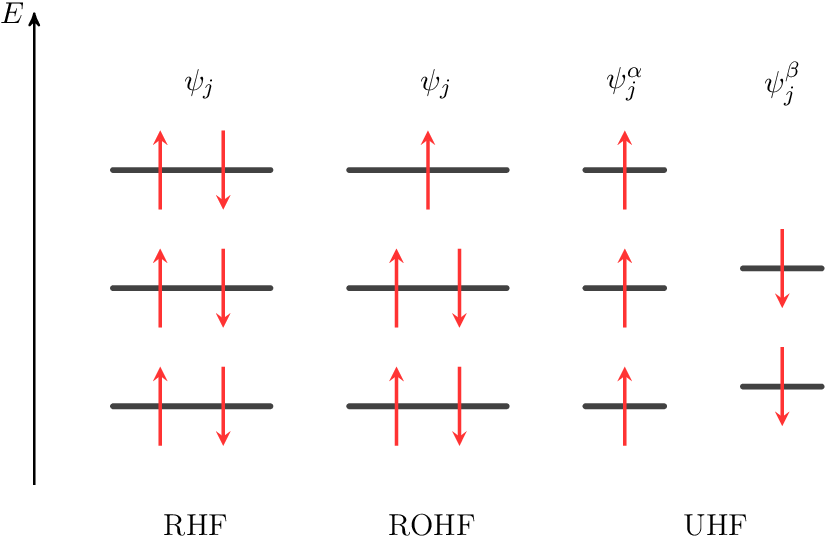
\includegraphics[width=0.5\linewidth]{Graphics/HF_Orb}
\caption{Différentes approches Hartree-Fock selon le remplissage électronique.}
\label{fig:hforb}
\end{figure}

\begin{itemize}
    \item \textbf{Hartree-Fock restreint (RHF - Restricted HF)}.
    \begin{itemize}
        \item Utilisé pour les systèmes où \textbf{toutes les orbitales occupées sont doublées} (couches fermées), c’est-à-dire que chaque orbitale moléculaire contient une paire d’électrons de spins opposés.
        
        \item Les mêmes fonctions spatiales sont attribuées aux électrons de spin $\alpha$ et $\beta$.
        
        \item Convient aux molécules dans un \textbf{multiplicité de spin singulet} ($S = 0$), comme les molécules diamagnétiques.
    \end{itemize}
    
    \item \textbf{Hartree-Fock restreint pour les couches ouvertes (ROHF - Restricted Open-Shell HF)}.
    \begin{itemize}
        \item Adapté aux molécules à \textbf{couches ouvertes}, où certains électrons ne sont pas appariés.
        
        \item Les orbitales occupées par deux électrons restent symétriques comme en RHF), tandis que les orbitales contenant un seul électron sont traitées de manière spécifique.
        
        \item Permet de modéliser des systèmes avec une \textbf{multiplicité de spin non nulle} ($S > 0$),  comme les radicaux ou les atomes ayant un moment magnétique net.
    \end{itemize}

    \item \textbf{Hartree-Fock non restreint (UHF - Unrestricted HF)}.
    \begin{itemize}
        \item Utilisé pour les systèmes à \textbf{couches ouvertes}, notamment lorsque le spin total du système ne permet pas une solution symétrique.
        
        \item Contrairement à RHF et ROHF, les électrons de spin $\alpha$ et $\beta$ sont décrits par des \textbf{fonctions spatiales différentes}.
        
        \item Permet une plus grande flexibilité mais peut introduire un phénomène d’\textbf{instabilité de spin} (le spin-contamination), où la solution obtenue ne correspond pas exactement à l’état de spin souhaité.
    \end{itemize}
\end{itemize}

\subsubsection{Comparaison et choix du modèle Hartree-Fock}

Le choix entre RHF, ROHF et UHF dépend du type de molécule étudiée :
\begin{itemize}
    \item \textbf{RHF} est adapté aux molécules \textbf{fermées} sans électron non-apparié (ex. \ch{H2}, \ch{CH4}).

    \item \textbf{ROHF} est souvent utilisé pour les systèmes avec \textbf{un nombre impair d’électrons} ou des \textbf{ions radicalaires} (ex. \ch{NO}, \ch{O2}).

    \item \textbf{UHF} est nécessaire pour les systèmes fortement magnétiques, où les électrons occupent des orbitales spatiales distinctes (ex. \textbf{métaux de transition, complexes paramagnétiques}).
\end{itemize}

Le tableau suivant résume les différences entre ces trois méthodes :

\begin{table}[h!]
    \centering
    \begin{tabular}{|l|c|c|c|}
        \hline
        \textbf{Méthode HF} & \textbf{Systèmes adaptés} & \textbf{Description des orbitales} & \textbf{Multiplicité de spin} \\
        \hline
        RHF  & Couches fermées & Identiques pour $\alpha$ et $\beta$ & $S=0$ \\
        \hline
        ROHF & Couches ouvertes (électrons non appariés) & Identiques sauf pour les non-appariés & $S>0$ \\
        \hline
        UHF  & Systèmes magnétiques/couches ouvertes & Différentes pour $\alpha$ et $\beta$ & $S>0$ \\
        \hline
    \end{tabular}
    \caption{Comparaison des méthodes Hartree-Fock selon la structure électronique.}
\end{table}

En pratique, UHF est souvent préféré pour des \textbf{états excités ou fortement corrélés}, tandis que RHF et ROHF sont plus appropriés pour les calculs standards d’énergie fondamentale.

\subsection{Quelques limites des méthodes HF}

La méthode de Hartree-Fock présente certaines limites :
\begin{enumerate}
\item \textbf{Approximation du champ moyen}. La corrélation électronique est uniquement prise en compte par l’interaction d’échange.
\item \textbf{Absence de corrélation électronique dynamique}. Les interactions instantanées entre électrons ne sont pas modélisées.
    \item \textbf{Difficultés pour les systèmes fortement corrélés}. La méthide de HF est inefficace pour les molécules avec liaisons multiples ou états multi-déterminants.
\item \textbf{Sensibilité aux bases de fonction}. La précision des résultats de la méthode de HF dépend fortement du choix des bases de fonction utilisées pour décrire les orbitales électroniques.
\end{enumerate}

\section{Choix de l'ensemble de bases}

L'équation de Schrödinger à plusieurs électrons est généralement résolue sur une base d'orbitales moléculaires exprimées sous la forme d'une \textbf{combinaison linéaire de ses orbitales atomiques (LCAO, Linear
combination of atomic orbitals)}, 
\begin{equation}
     \phi_a(\mathbf{r}) =
     \sum_A^\mathrm{atomes}
     \sum_\alpha C^A_{\alpha a}
     \chi^A_{\alpha}(\mathbf{r} - \mathbf{R}_A) .
\end{equation}
où $\chi^A_{\alpha}(\mathbf{r} - \mathbf{R}_A)$ sont les \textbf{fonctions de base} centrées sur l’atome $A$, et $C^A_{\alpha a}$ sont les coefficients de la combinaison linéaire. Ces coefficients sont optimisés via le \textbf{principe variationnel}.

\subsection{Ensembles de bases traditionnels}

Les deux classes principales d'orbitales de base approximatives utilisées en chimie quantique sont :
\begin{itemize}
\item les \textbf{Slater-type orbitals (STOs)} basées sur le déterminant de Slater, construitent avec des fonctions exponentielles décroissantes
    \begin{equation}
        \chi_{\mathrm{STO}}(r) = e^{-\alpha r},
    \end{equation}
\item et les \textbf{orbitales cartésiennes de type Gaussien (GTO)}, construitent avec des fonctions Gaussiennes
    \begin{equation}
        \chi_{\mathrm{GTO}}(r) = e^{-\alpha r^2}.
    \end{equation}
  Ces orbitales facilitent le calcul des intégrales de recouvrement et sont donc plus couramment utilisées que les STO en chimie quantique computationnelle.
\end{itemize}

Les STO sont plus proches de la forme exacte des orbitales atomiques, mais les GTO permettent de simplifier les calculs d’intégrales électroniques. Un compromis entre ces deux approches consiste à combiner plusieurs GTO pour approximer une STO, donnant naissance aux bases \textbf{STO-nG} (Slater-Type Orbital – n Gaussians), où $n$ est le nombre de Gaussiennes utilisées dans l’approximation.

\subsection{Notations des ensembles de bases}

Les ensembles de bases sont constitués de plusieurs \textbf{primitives gaussiennes}. L'une des notations les plus explicites est celle de Pople :
\begin{itemize}
    \item Le \textbf{trait d'union (-)} sépare la référence aux orbitales centrales et de valence ;
    \item Les \textbf{chiffres} indiquent le nombre de primitives Gaussiennes utilisées ;
    \item La \textbf{lettre G} signifie que des Gaussiennes sont utilisées.
\end{itemize}

Par exemple, la base \texttt{6-31G} signifie :
\begin{itemize}
    \item 6 primitives Gaussiennes pour les orbitales internes.
    \item 3 primitives Gaussiennes pour les orbitales de valence.
    \item 1 primitive supplémentaire pour améliorer la flexibilité.
\end{itemize}
Cette notation s’étend aux bases plus complexes, comme \texttt{6-31G(d,p)}, où \textbf{(d,p)} indique l’ajout de fonctions de polarisation sur certains atomes.

En parallèle, d'autres familles d’ensembles de bases ont été développées pour répondre à des besoins spécifiques, notamment en méthodes post-Hartree-Fock.

\subsection{Bases correlation-consistent}

Les méthodes de chimie quantique avancées nécessitent des bases capables de capturer les effets de \textbf{corrélation électronique}. La famille \texttt{cc-pVXZ} (\textit{correlation-consistent polarized valence X-zeta}) est spécifiquement conçue pour cela :
\begin{itemize}
    \item \texttt{cc-pVDZ} : Double-$\zeta$, bonne précision pour les calculs préliminaires.
    \item \texttt{cc-pVTZ} : Triple-$\zeta$, plus précis pour les corrélations électroniques.
    \item \texttt{cc-pVQZ} : Quadruple-$\zeta$, nécessaire pour des énergies précises.
    \item \texttt{aug-cc-pVDZ} : Ajout de fonctions diffuses pour mieux représenter les anions et les états excités.
\end{itemize}

Plus d'informations, d'exemples et de discussions sur les GTO peuvent être trouvés dans ce
\href{https://chem.libretexts.org/Courses/Pacific_Union_College/Quantum_Chemistry/11\%3A_Computational_Quantum_Chemistry/11.02\%3A_Gaussian_Basis_Sets}{lien}.

\subsection{Catégories d'ensembles de bases}

Les ensembles de bases modernes se répartissent en plusieurs catégories,
chacune adaptée à des besoins spécifiques en termes de précision et de coût
computationnel. Le tableau \ref{tab:basis_sets} résume les principales familles.

\begin{table}[h!]
    \centering
    \begin{tabular}{|l|p{8cm}|p{3cm}|}
        \hline
        \textbf{Catégorie} & \textbf{Description} & \textbf{Exemple} \\
        \hline
        Minimale & Une seule fonction de base par orbitale atomique occupée. & STO-3G \\
        \hline
        Double-$\zeta$ & Deux fonctions de base par orbitale atomique de valence. & 6-31G \\
        \hline
        Triple-$\zeta$ & Trois fonctions de base par orbitale atomique de valence. & 6-311G \\
        \hline
        Polarisation & Ajout de fonctions d'ordre supérieur pour mieux représenter la flexibilité des orbitales. & cc-pVDZ \\
        \hline
        Diffusion & Utilisation de fonctions étendues pour modéliser des électrons faiblement liés ou des états excités. & 6-31+G, aug-cc-pVDZ \\
        \hline
    \end{tabular}
    \caption{Différentes catégories d'ensembles de bases utilisées en chimie quantique.}
    \label{tab:basis_sets}
\end{table}

\subsection{Bases de Karlsruhe}

Les ensembles \texttt{def2} de Karlsruhe offrent une alternative moderne aux bases de Pople et correlation-consistent. Elles couvrent l’ensemble du tableau périodique jusqu’au radon ($Z=86$) et intègrent des
\textbf{potentiels de noyau effectif (ECP)} pour les éléments lourds. Trois niveaux de précision sont disponibles :
\begin{itemize}
    \item \textbf{def2-SVP} : Base compacte, adaptée aux calculs rapides (équivalent à \texttt{6-31G**}).
    \item \textbf{def2-TZVP} : Triple-$\zeta$ avec polarisation, bon compromis précision/coût.
    \item \textbf{def2-QZVP} : Quadruple-$\zeta$, utilisé pour des études très précises.
\end{itemize}
L'utilisation de bases \texttt{def2} est souvent privilégiée en \textbf{DFT (Density Functional Theory)} et en \textbf{calculs post-Hartree-Fock}.

\subsection{Critères pour choisir un ensemble de bases}

Le choix optimal dépend du système étudié et des exigences du calcul. En règle générale pour,
\begin{itemize}
    \item \textbf{Études rapides :} \texttt{6-31G}, \texttt{def2-SVP}.
    \item \textbf{Chimie de la valence :} \texttt{cc-pVDZ}, \texttt{def2-TZVP}.
    \item \textbf{Calculs précis :} \texttt{cc-pVTZ}, \texttt{def2-QZVP}.
    \item \textbf{Anions et états excités :} \texttt{aug-cc-pVDZ}, \texttt{def2-TZVPPD}.
    \item \textbf{Effets relativistes :} bases avec \textbf{potentiels de noyau effectif (ECP)}, ex. \texttt{LANL2DZ}.
\end{itemize}

En augmentant la taille de l’ensemble de bases, l’approximation obtenue  se rapproche de la fonction d’état exacte :
\begin{equation}
\langle \Phi_{\text{approx}} | \mathtt{H} | \Phi_{\text{approx}} \rangle \geq  \epsilon_{\text{true}}.
\end{equation}
Cependant, une base plus grande implique une augmentation des coûts de calcul. Il est donc essentiel de trouver un équilibre optimal.

\subsection{Conclusion}

Le choix d’un ensemble de bases est un facteur déterminant en chimie quantique computationnelle. Un compromis doit être trouvé entre la précision souhaitée et les ressources disponibles.
Les bases modernes, comme \texttt{def2} et \texttt{cc-pVXZ}, offrent des solutions flexibles adaptées à divers niveaux de calcul. En sélectionnant soigneusement une base appropriée, on optimise le rapport coût-précision pour les études moléculaires.


\end{document}
